%% LyX 2.0.0 created this file.  For more info, see http://www.lyx.org/.
%% Do not edit unless you really know what you are doing.
\documentclass[english,journal]{IEEEtran}
\usepackage[T1]{fontenc}
\usepackage[latin9]{inputenc}
\usepackage{babel}
\usepackage{textcomp}
\usepackage{amssymb}
\usepackage{graphicx}
\usepackage[unicode=true]
 {hyperref}
\usepackage{breakurl}

\makeatletter
%%%%%%%%%%%%%%%%%%%%%%%%%%%%%% User specified LaTeX commands.

\usepackage{array}\usepackage{subfigure}


\newcolumntype{x}[1]{%
 {\centering\hspace{Opt}}P{#1}}%
\newcommand{\tn}{\tabularnewline}

\makeatother

\begin{document}

\title{Idle Injection Mechanism Implemented in\\
the BFS scheduler}


\author{Andrea Mambretti, \emph{student id: 783286}\\
Luca Muccignato, \emph{student id: 783274}}
\maketitle
\begin{abstract}
In these days the problems of power consumpion and temperature management
have become two of the most studied fields in computer architecture.
Lots of applications are built with different methods and different
levels of abstraction to try to manage them. Various techniques are
implemented at the hardware level, others are at software level either
in the kernel or in userspace.

In this paper we want to discuss about the concepts, implementation
and results of a system based on the BFS scheduler of Linux that uses
the \underline{idle injection method} to reduce the workload and
therefore the temperature of a stressed system. This kind of solution,
as you will undestand, has already been used and implemented on other schedules, but there's
nothing similar for that kind of scheduler. 
\end{abstract}
\begin{keywords}Operative System, Linux Kernel, Power Consumption,
Temperature, Scheduling, Idle Injection \end{keywords}


\section{INTRODUCTION}

In modern computer architecture, developers are obliged to consider
the problems caused by high temperature and power consumpion. These
can really have a bad impact on the performance of a system, in terms
of throughput and overheating of components.

To avoid this situation, we can work at hardware level using more
parallelized cores, processor with multithreading support, "do nothing well"
technique, lower power state for DRAM or disks and dynamic voltage
frequency scaling.

However, we can also work at software level using idle injection or
frequency scaling techniques. Today, more or less all modern CPUs
have the Frequency Scaling Support, which is used by the operative
system to control the power consumpion (they have policy like powersave,
ondemand etc), whereas there are only few implementations of idle
injection technique.

In this paper we will present our own solution for the linux kernel
3.2.6 patched with the BFS scheduler by Con Kolivas. The background chapter
is an overview on the situation of the modern schedulers in
the linux kernel. The following chapter (the heat problem) describes the temperature problem and the possible consequences. The fourth chapter talks about the aims of our project and the theoric concept of our solution. The fifth chapter describes the implementation details and then there is a chapter about the results we obtained, with a short description of our three tests. In the end, we make an overview of possible future works related to our project. 


\section{BACKGROUND}

In today linux boxes, we can find two main versions of the scheduler.
One is in the mainline of linux kernel, created by Ingo Molnar and
called CFS; the other is an unofficial version, developed autonomously
by Con Kolivas, after an argue with Molnar\cite{key-1}, and called
BFS.\medskip{}


CFS\cite{key-6}, which stands for Completely Fair Scheduler, is in
the mainline since 2007. The idea behind is based on the Fair-Share
Scheduling policy, which divides the CPU time among entities, such
as users, groups, or tasks. CFS can support all this levels, but was
originally created for scheduling at task level. Each one of these tasks
should have a fair share of the CPU, but this is an ideal case. CFS
keeps track of how much time is given to a task respect the others,
so it can schedule the one with the highest level of unfairness. To
easily know which task it should choose, CFS organizes them in a red-black
tree, descending ordered by their total unfairness. The chosen task
is the leftmost and the total time required to schedule it is $O\left(\log n\right)$,
where n is the number of tasks present in the system. When the current
task has finished running on the CPU, just before selecting the new
one, the scheduler increments the task's \textit{vruntime} field,
which saves the amount of time that the CPU has dedicated to it. Then
the scheduler chooses the most unfairly treated task by selecting the
one with the lowest vruntime. At its creation, a new task is given
the minumum value of current vruntime, which is stored and mantained
in a variable in order to speed up the whole process. So, there is
no concept of timeslice, but a task runs until it's no longer the most
unfairly treated. In order to reduce the context switching overhead
(the time used for sending a content switch signal), CFS introduces
a minimum granulrity of time (a minimum time that a chosen task must
at least run), used to control the tradeoff between latency and content
switching's overhead. In case of multiprocessor architectures, CFS
keeps separate data structures for each CPU, reducing lock contention
but requiring some sort of load balancing to spread tasks across processors.

BFS\cite{key-2}, which stands for Brain Fuck Scheduler, was written
by Kolivas as an alternative to CFS. It doesn't adopt the modular
framework of CFS; instead it uses one single system-wide runqueue,
containing all non-running tasks. In this way, it's able to determine
the next scheduled task without using some sort of special and complicated
heuristic. BFS implements an earliest effective virtual deadline policy.
A virtual deadline is the ideal time that any two tasks with the same
niceness will have to wait before running on the CPU; when a task asks for CPU usage, it is assigned a deadline. Even if the deadline is virtual, because there is no assurance that a task will be scheduled
by that time, however tasks will be scheduled from earlier to later
virtual deadlines. Because of this approach, earlier virtual deadlines
are given to tasks with higher priority. If a task blocks, it keeps
the remainder of its timeslice and virtual deadline, so it gains higher
priority when is rescheduled. Because of there is no order of tasks
in the runqueue, they cannot be placed in a tree like in CFS' solution
and the lookup for the next scheduled task takes an $O\left(n\right)$
scan over the whole queue. As a consequence, BFS scales poorly with
large amounts of tasks. Furthermore, a share data structure among
all CPUs increases lock contention, but tasks can be quickly scheduled
on different CPUs without problems as soon as they become available.
This results in a lower latency.\medskip{}
 On the net it is possible to find several stress tests, even if only
few of them really explanatory\cite{key-7}, made using benchmarking
programs, like latt.c a tool specific for schedulers's benchmarking,
or just using gcc instruction, make for example, or playing a video.
All tests can be done on netbook, laptop and desktop, too. Results
generally demonstrate that BFS scheduler has a lower latency, which
is not a surprise indeed as it was written with this aim. However
CFS scheduler results have a better performance in terms of turnaround
time (which is the total time taken between the submission of a task
for execution and the return of the output) under different load conditions,
especially with multicore machines. Finally, another result is that
BFS scheduler, playing a video, drops much less frames than CFS, under
large amounts of load.

As a conclusion, we can say that, generally, CFS is better in terms
of turnaround time, and so for batch processing, while BFS has a less
latency, more indicated for interactive tasks.


\section{THE HEAT PROBLEM}

More than in the past years, heat is a main problem that must be taken
into account while building systems. Components are susceptible to
malfunction or even break if overheated, especially integrated circuits
like CPUs. Because of these problems, components are often designed to generate
as little heat as possible and operating systems try to reduce power
consumption which generates heat. In modern computers, integrated
circuits are the prime source of heat, due to the fact that they work
at high frequency and voltage. Increasing CPUs workload in order to
exploit better performance in term of thrughput and speed up, with i.e.
ILP, results, as a drowback, in an increasing amount of warmth
produced by components.

Nowadays all CPUs and GPUs must use dedicated Heat Sinks or they will
reach high temperatures in few time of work. But there is the possibility to reduce it also via software, by writing programs properly, using specific software or solutions that involve idle injection, as well.\medskip{}


Because it's the mainline kernel, proposals in this last way are already
provided for CFS scheduler. One, for example, is Kidled by Google,
which scope is to realize a power capping through idle cycle injection\cite{key-8}.
It consists in a module for the CFS scheduler, patched by Google developer
Salman Qazi\cite{key-9}, which allows the system administrator to
set the percentage of time that a specific CPU should be idle and
an interval over which that percentage is calculated. To avoid important
processes to be stalled, there is the special notation "interactive"
with which a process can be marked and, when running, idle cycles
will be forced only when necessary. Kidled code also allows system
administrator to select a process that should be idled, so he can
chooses if he wants to affect all the system or just a single process.
The result is a reduction of power consumption and, as a consequence,
a reduction of heating.


\section{SYSTEM GOAL AND APPROACH}

The goal of our system is to provide an injection control mechanism
of idle cycles for the linux BFS kernel which is able to reduce the
power consumpion and the average temperature. The aim of doing that
is to try to maintain the best condition of work, in terms of heating,
also when a system is overloaded. To garantee the flexibility and
the usability, our system has no policy hardcoded inside, whereas
there are two interfaces where external monitors can plug in and control
them specifing their own policies.

Another use that can be done with this system is to control a process
or thread's throughput, injecting more or less idle cycles during
its specific execution, to keep its performance in a defined range.\medskip{}


Our approch is based on the behaviour of the scheduler. We mainly
worked on the \textit{schedule() }function, the one that chooses the
earliest deadline task. The idea behind our system is to inject idle
every X calls of the \textit{schedule() }function, or Y times that
a specific process is scheduled. We faked the condition inside the
BFS to force it to schedule an idle cycle, instead of the elected
process. The way is to change, if needed, the \underline{next} process
with the idle process before that the \textit{context\_switch function}
is called. Actually, our system doesn't consider realtime processes
because it has no much sense to work on a process that needs all the
resources given to it.\medskip{}


Our implementation provides two main functions, one which works globally
on the machine and the other one on a specific process or thread (via
its identifier, pid or tid).

The global function can be used to keep under control the temperature
of the machine when it's rising.

The second function works on a specific identifier that can be used
to control a single process or a thread (even more than one at a time),
maybe because it's requiring more CPU time respect to the amount that
we want to give it (ex. updates manager). 

Our system has two interfaces, working through procfs, which either
the user directly or a monitor program as well can use to control
the injection (see the Implementation Chapter below).

We realized a monitor program as a test that uses a simple heuristic to control
the quantity of idle cycles injected, based on current heat (the higher
is the temperature, the greater is the number of cycles injected), but other
monitors can be attached.

On the other hand, if an user wants to administrate the number by him or herself, he or she can do it freely.


\section{IMPLEMENTATION}

In this section we want to present some more detailed aspects of our
own implementation.\medskip{}



\subsection{IDLE PROCESS}

Our mechanism is an injector of idle, but what is an idle process?
Actually it can be different things.

In some cases it is a process with pid=0 that executes a sequence
of NOP instructions and it is scheduled if and only if there isn't
any other process that can execute (it's the process with the lowest
priority). In other cases it indicates a turned off cpu, switched
off to save power when it has nothing to execute.

Inside the linux kernel, an idle is like a normal process that does
nothing; it's the only process where the \emph{task\_struct} isn't
dynamically allocated, but is statically defined at kernel build time
and is called init\_task.

We decide to use this special process because it's already defined
for the kernel and makes the processor doing exactly what we want
it to do, that is nothing.\medskip{}



\subsection{CHANGES TO THE OPERATING SYSTEM}

The linux version's choice is totally arbitrary for using our system.
In our own implementation we choose Gentoo, with a standard \emph{kernel
3.2.6}%
\footnote{Actually the system works for sure only on this version but maybe
it can also works with previous version of the kernel.%
}.

That kernel was patched with a Kovalis' patch porting made by us. We
also performed another patch with the HRM system, used to get details
about the impact on the thoughput of our application. Finally, we
had to install the lm\_sensors module to get information from the
temperature sensors.\medskip{}



\subsection{GLOBAL INJECTION}

The global injection is realized to take under control the global
scheduling machanism. The point where we modified the schedule to
achive this kind of injection is just inside the \textit{schedule()}
function.

The number of calls to this function that can be done before an idle
is executed is variable and can be modified via procfs, using a file
which can be found in \emph{/proc/schedidle/sched\_global}. The monitor
does it automatically, trying to keep the temperature at about 60\textdegree{}C,
while an user, to insert a specific new value, can simply use an echo
into this file, overwriting the current X quantity%
\footnote{Ex. If an user writes on terminal "echo 200 \textgreater
/proc/schedidle/sched\_global", it means that every
200 calls of schedule() an idle cycle is executed.

Keep in mind that, for doing so, Monitor program must be stopped
or it will overwrite user's value with the one prefixed.%
}.

Using this kind of injection it's possible to apply different type
of policy, starting from a simple one that only checks the global
heat (calculating the average temperature of the cores) and ending
with a more complex policy that takes into account also other metrics
like the cpu's workload.

We tested it with the simple metric that takes into account only the
average temperature of the testing machine (see Results Chapter).\medskip{}



\subsection{PID/TID CONTROL}

The second implementation is a finer mechanism used to control
processes or threads. As before, the point where we modified the schedule
to achieve this kind of injection is just inside the \textit{schedule()}
function.

The system uses a file in procfs whose path is \emph{/proc/schedidle/sched\_pid.
}\textit{\emph{As in the Global Injection,}}\textit{ }either an user
or the monitor program can access to it and control the injection's
frequency. Managing this file, a list inside the kernel
space is updated, where tuples with the following information are stored:
\begin{enumerate}
\item Identifier: number that tells to the kernel which process/thread to control. 
\item Y: this value means "put an idle process every Y times
that the process with pid/tid = identifier is executed".
\item Type: this field says if the identifier refers to either a process
or a thread. Its value can be equal to p or t.
\end{enumerate}
Also there the user can add a specific process or thread manually,
using an echo on the file above%
\footnote{Ex. If an user writes on terminal "echo 1000,6,p \textgreater
/proc/schedidle/sched\_pid", it means that an idle cycle
is executed instead of the process with pid equal to 1000 every 6 times
that that process is scheduled.%
}.


\section{RESULTS}

We tested our own implementation in three different ways which are
made to cover and verify the main goals of our injector.

The first is realized in order to show how we can control the temperature
of the machine under stress.

The second shows how the throughtput decrease unsing the control on
threads.

The third is done to control the maximum throughtput of the system
injecting, when needed, some idle cycles.

The testing enviroment is a Dell Laptop xps m1330 version with an
Intel Core2 Duo T7100. As said before we installed a Gentoo linux
with our own patched kernel version. Our tests use the HRM monitor
to see which is the throughput of our groups of threads and they use
the lm\_sensors to monitor the temperatures.

Now let's get a more deeply look on each test.\medskip{}



\subsection{Global Temperature Management\medskip{}
}

The idea behind this test is to show how a simple monitor can manage
the temperature of an overloaded laptop.

To do so, we modified the "sensors" tool
available in lm\_sensors so now it computes the average temperature
of the cores and, depending on the result, it changes the rate inside
the sched\_global file in procfs that says how much idle the system
has to inject.

The figure below shows our results:\medskip{}


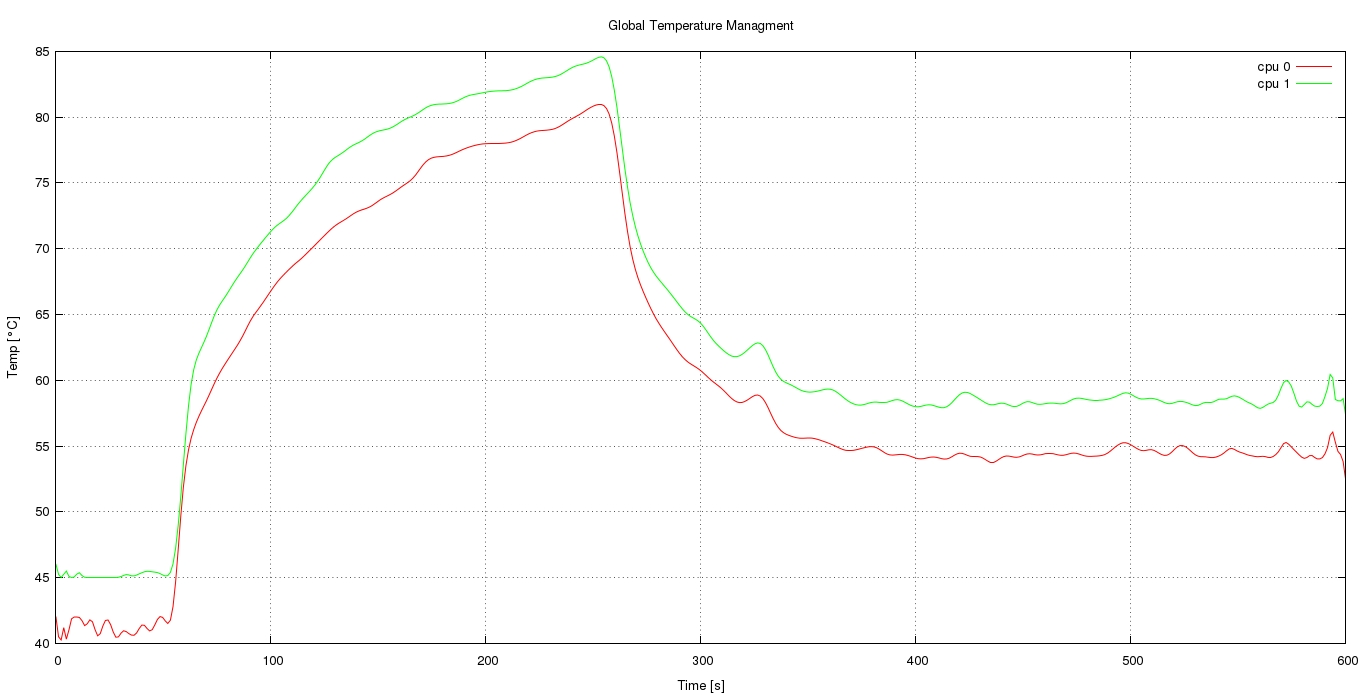
\includegraphics[scale=0.175]{Global_Temperature_Managment}

\medskip{}
This graph shows the effectiveness of using the system for managing
the whole temperature of a machine on which both processes and threads are running indistinctly.

We let the PC's heat growing for about 240 seconds until 80-85\textdegree{}C,
then the monitor program is started.

It immediately detects a temperature higher than the one that it is
supposed to maintain and starts to inject idle cycles.

As a result, we can see a sudden decrease of temperature (really huge
at first, because of the great number of idle cycles injected in function of the high temperature read)
and then it becomes quite stable around 55-60\textdegree{}C, which
is a temperature of stabilization empirically obtained from tests.

The time in which the temperature reaches this stabilization is affected
by the number of processes and threads currently running on the machine
(the greater is their number, the more time it's needed).

The difference of temperature between the two cores is probably related
to physical reasons of how those two processors are built or how the
workload is distributed on cores and not to our system.\medskip{}



\subsection{Throughput Management of Specific Threads\medskip{}
}

With this second test we want to show that our implementation can
really influence the throughput of an appointed process or thread.

For the demo, we used a process running two threads, one on each core.
We also had to use the HRM system to monitor the thread's throughput
and collect data.

The figure below shows our results:\medskip{}


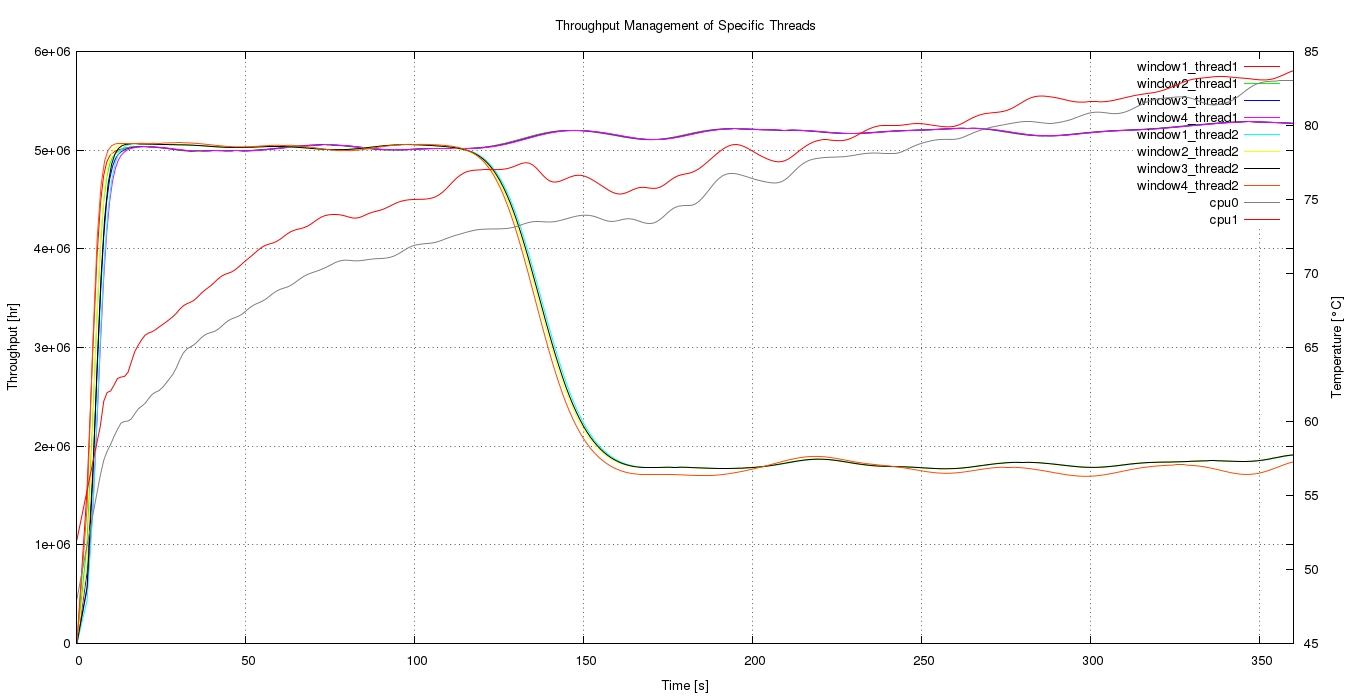
\includegraphics[scale=0.175]{Throughput_Management_of_Specific_Threads}

\medskip{}
Without going deeper, we can say that HRM program attaches 4 windows
to each pointed thread, in order to collect information from about
their throughputs. For this reason, we can see 4 windows linked to
thread1, running on CPU0, and 4 to thread2, running on CPU1. We firstly
let threads work normally, then, at about 120 seconds, we start idling
one of them, the one running on CPU1. This result is obtained injecting one idle every 5 executions of thread2

It's easy to see that its throughput decreases from $5*10^{6}$ heart rate to less than $2*10^{6}$ in really few time, just about
30 seconds.

Otherwise, thread1, which is not touched by our injection, continues
its execution with the same rate.

As a secondary result, we can notice that the temperatures of the
two cores tend to stabilize at a same value while, before injection,
CPU1 has an higher one. This is due to the fact that idles partly reduces
the overheating of that CPU. Because of this, we think that,
as a future work, it will be possible to add a function to our implementation,
in order to inject idles only on a single core and control its specific
temperature, instead of the machine's one (see the Current and Future
Works chapter below).\medskip{}



\subsection{Global Throughput Management}

In this last test we want to show how we can change the machine's
throughput, by injecting idles on the whole system. Again, we used
the HRM System to collect the final data. Here's the graph with our
results:\medskip{}
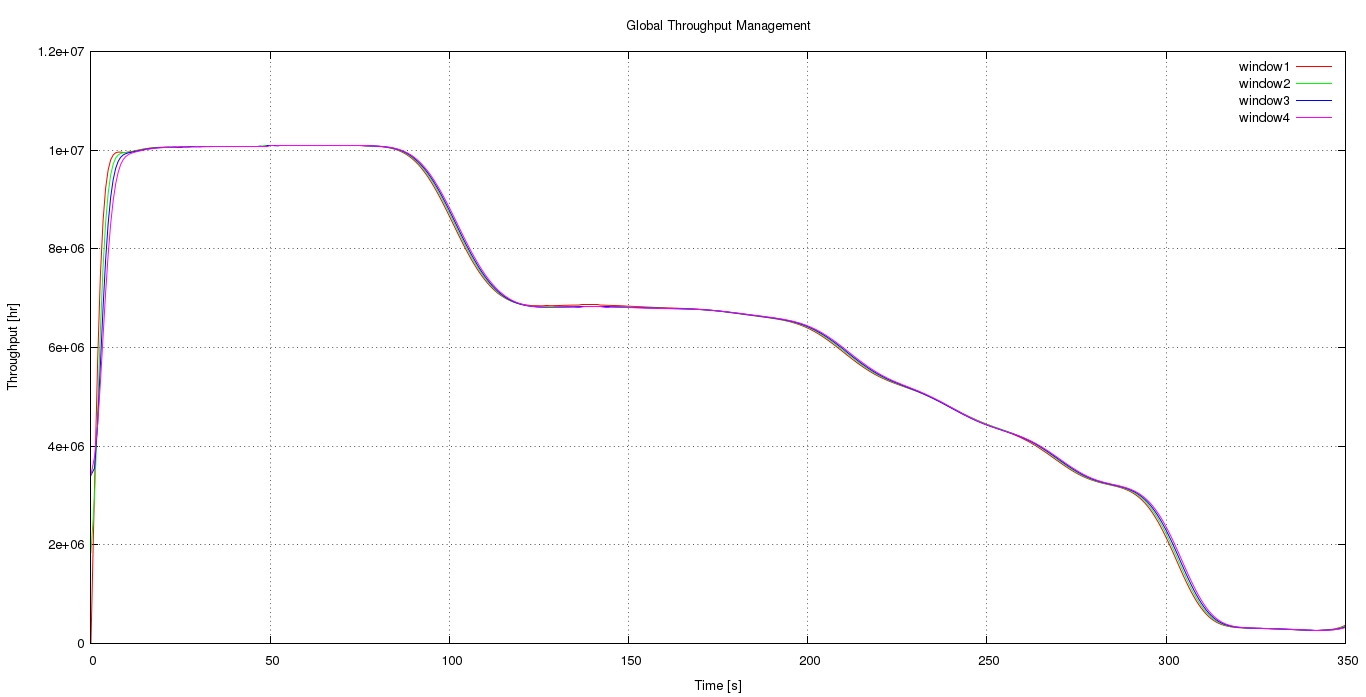
\includegraphics[scale=0.175]{Global_Throughput_Managment}

\medskip{}
As usual, we first let the PC work normally, then we start our monitor
program, this time modified to take under control the system's throughput.
It again uses a simple heuristic that inject more or less idles basing
on the current machine's performance, within a range. But this time,
we decided to increase the number of idle cycles executed if the throughput
is low, to show that we can bring it near zero.

In fact, we can see that the throughput strongly decreases when the
monitor is started after about 70 seconds, then it goes down linearly
until it reaches another range and again quickly falls.

Again we want to emphasize the fact that we could have stopped downing
the throughput at any time, we took it near zero for choice.

This case also gives an idea for a future improvement (see the Current
and Future Works chapter below). 


\section{CURRENT AND FUTURE WORKS}

The primary aim of our work is to help simple systems controlling their
temperature directly or modifing some processes throughput, as stated
several times before.\\
Secondly, our work can be a starting point for other interesting projects.

The first improvement that can be done is a Monitor which takes under
control the temperature and throughput with a policy that also considers
the number of processes running.

In addition, the Monitor should also treat the namespace number of
the processes to provide a finer grain. This can be used in
some kernel's versions (such as openvz) there's the possibility that
two processes may have the same pid/tid, due to the fact that they
belong to two different namespaces.

An easy improvement can be to provide the possibility to idle
a single core directly, not only just specific processes and threads running
on it or the global machine. As a result, we could be able to control
the temperature and throughput of an appointed core, which can be
useful for creating a differently-balanced architecture. Obviously
this makes sense only in a machine with many cores, placed on different
chips. This is because the core's temperature in a dual core PC where
CPUs are quite near can't differ so much.

Test case 3 also suggested the chance to create a mechanism able to
keep a core/process/thread's throughput in a stated range, calculated
alculated dinamically from the current system\textquoteright{}s state,
even with a simple heuristic. For example it can keep throughput X
in a range defined as 
\[
\frac{MST+mst}{2}*0.5\leqslant X\leqslant\frac{MST+mst}{2}*1.5
\]
 where MST is the maximum value of throughput of the system, mst the
minimum one. 

Finally, a nice challenge would be a porting of our project, to make
it able to run over other kind of schedulers.
\begin{thebibliography}{References}
\bibitem{key-1}Interview to Con Kolivas, why he quitted (even if he
came out with BFS 2 years after).\\
\href{http://apcmag.com/why_i_quit_kernel_developer_con_kolivas.htm}{http://apcmag.com/why\_{}i\_{}quit\_{}kernel\_{}developer\_{}con\_{}kolivas.htm}\medskip{}


\bibitem{key-6}What's CFS and its motivations on Red Hat.\\
\href{http://people.redhat.com/mingo/cfs-scheduler/sched-design-CFS.txt}{http://people.redhat.com/mingo/cfs-scheduler/sched-design-CFS.txt}\medskip{}


\bibitem{key-2}What's BFS and its motivations by Con Kolivas.\\
\href{http://ck.kolivas.org/patches/bfs/sched-BFS.txt}{http://ck.kolivas.org/patches/bfs/sched-BFS.txt}\medskip{}


\bibitem{key-7}Downloadable file comparing BFS and CFS by Taylor
Groves, Jeff Knockel and Eric Schulte.\\
\href{http://www.cs.unm.edu/~eschulte/data/bfs-v-cfs_groves-knockel-schulte.pdf}{http://www.cs.unm.edu/$\sim$eschulte/data/bfs-v-cfs\_{}groves-knockel-schulte.pdf}\medskip{}


\bibitem{key-8}Aim and basic ideas of Kidled. \\
\href{http://lwn.net/Articles/366775/}{http://lwn.net/Articles/366775/}\medskip{}


\bibitem{key-9}Patches provided by Salman Qazi.\\
Patch 0/3: \href{http://permalink.gmane.org/gmane.linux.kernel/973551}{http://permalink.gmane.org/gmane.linux.kernel/973551}\\
Patch 1/3: \href{https://lkml.org/lkml/2010/4/13/411}{https://lkml.org/lkml/2010/4/13/411}\\
Patch 2/3: \href{https://lkml.org/lkml/2010/4/13/412}{https://lkml.org/lkml/2010/4/13/412}\\
Patch 3/3: \href{https://lkml.org/lkml/2010/4/13/413}{https://lkml.org/lkml/2010/4/13/413}\end{thebibliography}

\end{document}
